\documentclass[aspectratio=169]{beamer}

\usetheme{Madrid}
\usecolortheme{default}
\usepackage{graphicx}
\usepackage{amsmath}

% Custom colors
\definecolor{meopblue}{RGB}{52, 152, 219}
\definecolor{meopred}{RGB}{231, 76, 60}

\setbeamercolor{title}{fg=white, bg=meopblue!80!black}
\setbeamercolor{frametitle}{fg=white, bg=meopblue!80!black}
\setbeamercolor{structure}{fg=meopblue!80!black}

\title{Power Dependence of MEOP Fit Parameters}
\subtitle{Cells C8 \& C9 --- 3\,W to 8\,W}
\author{MEOP Analysis}
\date{\today}

\begin{document}

% ---- Title slide ----
\begin{frame}
  \titlepage
\end{frame}

% ---- Slide 1: P0 vs Power ----
\begin{frame}{Decay Amplitude $P_0$ vs Laser Power}
  \begin{center}
    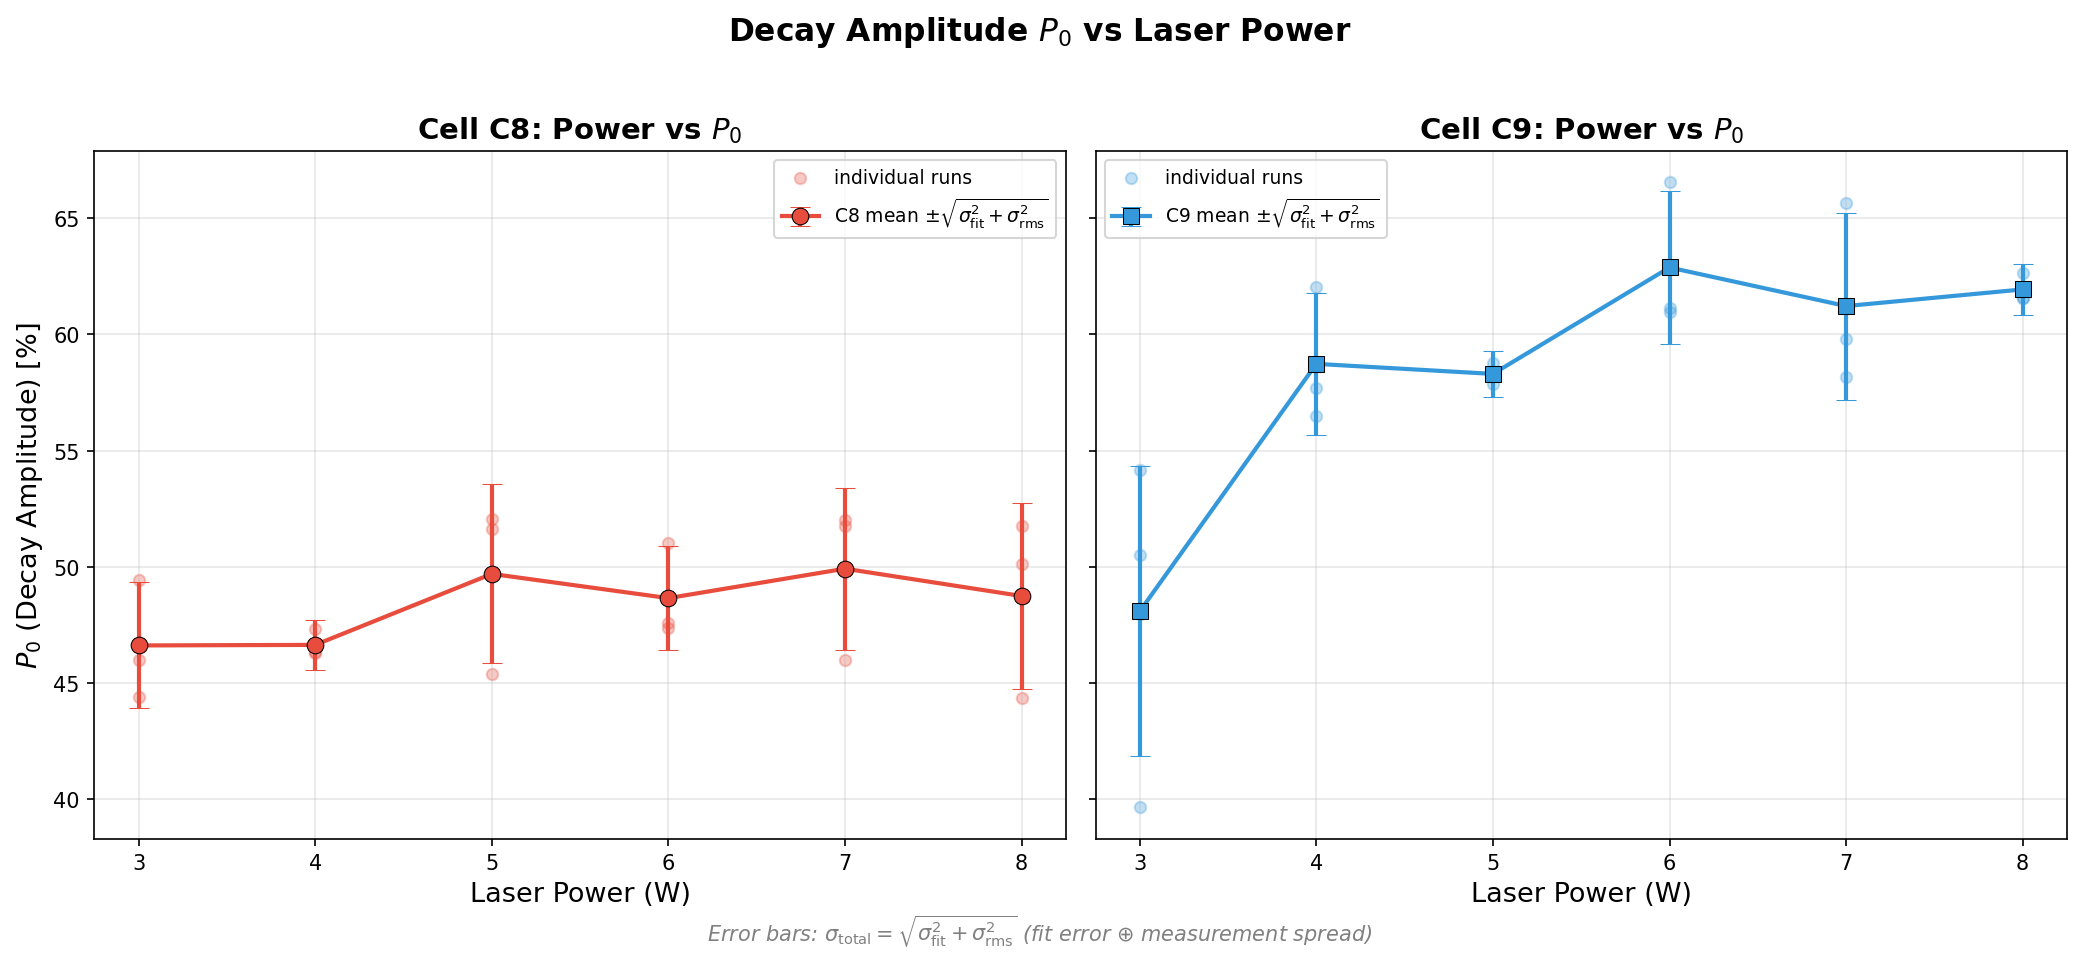
\includegraphics[width=0.75\textwidth]{power_vs_P0.png}
  \end{center}
  \vspace{-4mm}
  \footnotesize
  Error bars: $\sigma_{\mathrm{total}} = \sqrt{\sigma_{\mathrm{fit}}^2 + \sigma_{\mathrm{rms}}^2}$
  \hfill Faded points = individual datagrabs
\end{frame}

% ---- Slide 2: tau_b vs Power ----
\begin{frame}{Buildup Time Constant $\tau_b$ vs Laser Power}
  \begin{center}
    
\includegraphics[width=0.75\textwidth]{power_vs_tau_b.png}
  \end{center}
  \vspace{-4mm}
  \footnotesize
  Error bars: $\sigma_{\mathrm{total}} = \sqrt{\sigma_{\mathrm{fit}}^2 + \sigma_{\mathrm{rms}}^2}$
  \hfill Faded points = individual datagrabs
\end{frame}

% ---- Slide 3: tau_decay vs Power ----
\begin{frame}{Decay Time Constant $\tau_{\mathrm{decay}}$ vs Laser Power}
  \begin{center}
    
\includegraphics[width=0.75\textwidth]{power_vs_tau_decay.png}
  \end{center}
  \vspace{-4mm}
  \footnotesize
  Error bars: $\sigma_{\mathrm{total}} = \sqrt{\bar{\sigma}_{\mathrm{fit}}^2 + \sigma_{\mathrm{rms}}^2}$,\;
  $\bar{\sigma}_{\mathrm{fit}} = \sqrt{\sum\sigma_{\mathrm{fit},i}^2}/N$
  \hfill Faded points = individual datagrabs
\end{frame}

% ---- Slide 4: C8 vs C9 Comparison ----

\begin{frame}{C8 vs C9 Comparison}
  \begin{center}
    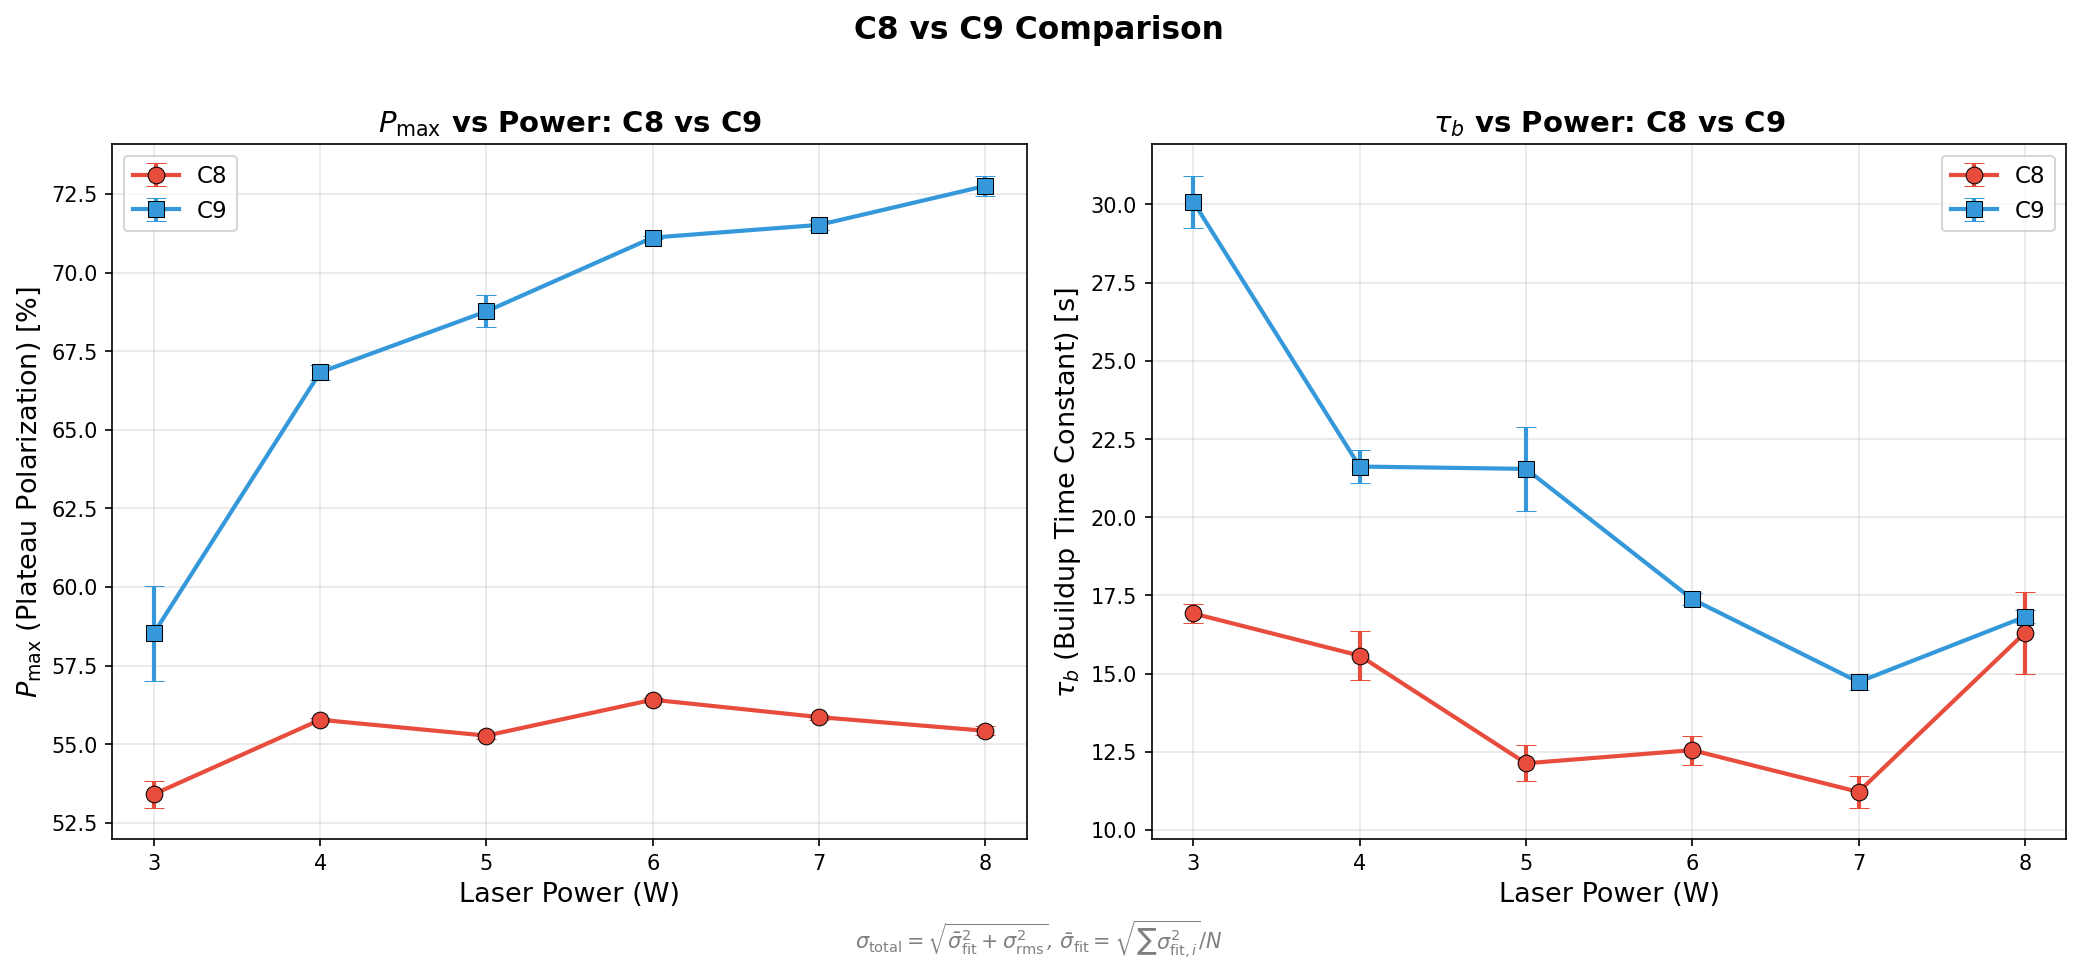
\includegraphics[width=0.75\textwidth]{C8_vs_C9_comparison.png}
  \end{center}
  \vspace{-4mm}
  \footnotesize
  \textcolor{meopred}{\textbullet\;C8} \quad
  \textcolor{meopblue}{\textbullet\;C9} \qquad
  Error: $\sigma_{\mathrm{fit}} \oplus \sigma_{\mathrm{rms}}$ added in quadrature
\end{frame}

% ---- Slide 5: Summary ----
\begin{frame}{Summary of Observations}
  \begin{columns}[T]
    \begin{column}{0.48\textwidth}
      \textbf{Decay Amplitude $P_0$}
      \begin{itemize}
        \item \textcolor{meopred}{C8}: Relatively flat ($\sim$47--50\,\%) across all powers
        \item \textcolor{meopblue}{C9}: Increases from $\sim$48\,\% (3\,W) to $\sim$63\,\% (6\,W), then plateaus
        \item C9 consistently higher than C8 above 4\,W
      \end{itemize}
    \end{column}
    \begin{column}{0.48\textwidth}
      \textbf{Buildup Time $\tau_b$}
      \begin{itemize}
        \item Both cells: $\tau_b$ decreases with increasing power (faster buildup)
        \item \textcolor{meopblue}{C9} starts much higher ($\sim$33\,s at 3\,W) vs \textcolor{meopred}{C8} ($\sim$17\,s)
        \item Convergence at high power ($\sim$16\,s at 8\,W)
      \end{itemize}
    \end{column}
  \end{columns}

  \vspace{6mm}
  \centering
  \footnotesize
  All error bars: $\sigma_{\mathrm{total}} = \sqrt{\sigma_{\mathrm{fit}}^2 + \sigma_{\mathrm{rms}}^2}$ \quad
  (fit uncertainty $\oplus$ run-to-run spread, independent errors)
\end{frame}

\end{document}
